\documentclass[notes,10pt, aspectratio=169]{beamer}

\usepackage{pgfpages}
% These slides also contain speaker notes. You can print just the slides,
% just the notes, or both, depending on the setting below. Comment out the want
% you want.
\setbeameroption{hide notes} % Only slide
%\setbeameroption{show only notes} % Only notes
%\setbeameroption{show notes on second screen=right} % Both
\usepackage{colortbl}
\usepackage{helvet}
\usepackage[default]{lato}
\usepackage{array}
\usepackage{eurosym}
\usepackage{setspace}
\usepackage{animate}
\usepackage{multicol}
\usepackage{breqn}
\usepackage{subcaption}
\usepackage{caption}
\captionsetup{font=scriptsize, justification=raggedright,singlelinecheck=false}
\usepackage[export]{adjustbox}
\usepackage[scale=2]{ccicons}
\usepackage{tikz}
\newenvironment{wideitemize}{\itemize\addtolength{\itemsep}{10pt}}{\enditemize}
\usepackage{natbib}

\usepackage{tikz}
\usepackage{verbatim}
\setbeamertemplate{note page}{\pagecolor{yellow!5}\insertnote}
\usepackage{amsmath}
%\usepackage{mathpazo}
\usepackage{hyperref}
\usepackage{lipsum}
\usepackage{multimedia}
\usepackage{multirow}
\usepackage{graphicx}
\usepackage{dcolumn}
\usepackage{bbm}
\newcolumntype{d}[0]{D{.}{.}{5}}

\usepackage{changepage}
\usepackage{appendixnumberbeamer}
% \newcommand{\beginbackup}{
%   \newcounter{framenumbervorappendix}
%   \setcounter{framenumbervorappendix}{\value{framenumber}}
%   \setbeamertemplate{footline}
%   {
%      \leavevmode%
%      \hline
%      box{%
%       \begin{beamercolorbox}[wd=\paperwidth,ht=2.25ex,dp=1ex,right]{footlinecolor}%
% %         \insertframenumber  \hspace*{2ex} 
%       \end{beamercolorbox}}%
%      \vskip0pt%
%   }
%  }

 \setbeamertemplate{footline}{
    \hbox{%
    \begin{beamercolorbox}[wd=\paperwidth,ht=3ex,dp=1.5ex,leftskip=2ex,rightskip=2ex]{page footer}%
        %\usebeamerfont{title in head/foot}%
        %\insertshorttitle \hfill
        %\insertsection \hfill
        %\tableofcontents[currentsection] \hfill
        \insertsectionnavigationhorizontal{0.7\paperwidth}{}{} \hfill 
        \insertframenumber{} / \inserttotalframenumber
    \end{beamercolorbox}}%
}
\newcommand{\backupend}{
   \addtocounter{framenumbervorappendix}{-\value{framenumber}}
   \addtocounter{framenumber}{\value{framenumbervorappendix}} 
}

\useinnertheme[shadow]{rounded}
\setbeamercolor{block title example}{fg=black,bg=orange!50!white}
\setbeamercolor{block body example}{fg=black, bg=orange!30!white}
\setbeamercolor{block title}{use=structure,fg=structure.fg,bg=structure.fg!20!bg}
\setbeamercolor{block body}{parent=normal text,use=block title,bg=block title.bg!50!bg}

\newcommand\independent{\protect\mathpalette{\protect\independenT}{\perp}}
\def\independenT#1#2{\mathrel{\rlap{$#1#2$}\mkern2mu{#1#2}}}

\usepackage{graphicx}
\usepackage[space]{grffile}
\usepackage{booktabs}

% These are my colors -- there are many like them, but these ones are mine.
\definecolor{blue}{RGB}{0,114,178}
\definecolor{red}{RGB}{213,94,0}
\definecolor{yellow}{RGB}{240,228,66}
\definecolor{green}{RGB}{0,158,115}

\setbeamercolor{section in head/foot}{fg=blue}


\hypersetup{
  colorlinks=false,
  linkbordercolor = {white},
  linkcolor = {blue}
}


%% I use a beige off white for my background
\definecolor{MyBackground}{RGB}{255,253,218}

%% Uncomment this if you want to change the background color to something else
%\setbeamercolor{background canvas}{bg=MyBackground}

%% Change the bg color to adjust your transition slide background color!
\newenvironment{transitionframe}{
  \setbeamercolor{background canvas}{bg=yellow}
  \begin{frame}}{
    \end{frame}
}

\setbeamercolor{frametitle}{fg=blue}
\setbeamercolor{title}{fg=black}
%\setbeamertemplate{footline}[frame number]
\setbeamertemplate{navigation symbols}{} 
\setbeamertemplate{itemize items}{-}
\setbeamercolor{itemize item}{fg=blue}
\setbeamercolor{itemize subitem}{fg=blue}
\setbeamercolor{enumerate item}{fg=blue}
\setbeamercolor{enumerate subitem}{fg=blue}
\setbeamercolor{button}{bg=white,fg=blue,}



% If you like road maps, rather than having clutter at the top, have a roadmap show up at the end of each section 
% (and after your introduction)
% Uncomment this is if you want the roadmap!
% \AtBeginSection[]
% {
%    \begin{frame}
%        \frametitle{Roadmap of Talk}
%        \tableofcontents[currentsection]
%    \end{frame}
% }
\setbeamercolor{section in toc}{fg=blue}
\setbeamercolor{subsection in toc}{fg=red}
%\setbeamersize{text margin left=1em,text margin right=1em} 
\setbeamersize{text margin left=0.7cm,text margin right=0.7cm} 


\title[]{\textcolor{blue}{Lecture 6 v2:\\Inference and Interpretation}}
\author{25117 - Econometrics}
\institute[shortinst]{Universitat Pompeu Fabra}

\date{October 23rd, 2024}

\begin{document}

\begin{frame}[plain]
\maketitle
\end{frame}


\begin{frame}{What we learned in the last lesson}
\begin{itemize}
    \item Omitted variable bias occurs when an omitted variable (a) is correlated with an included regressor and (b) is a determinant of $Y$.\\[1em]
    \item The multiple regression model is a linear regression model that includes multiple regressors, $X_1, \dots, X_k$. Associated with each regressor is a regression coefficient, $\beta_1, \dots, \beta_k$.\\[1em]
    \item The coefficient $\beta_1$ is the expected difference in Y associated with a one-unit difference in $X_1$, holding the other regressors constant. The other regression coefficients have an analogous interpretation.\\[1em]
\end{itemize}
\end{frame}

\begin{frame}{What we learned in the last lesson}
\small
\begin{itemize}
    \item Throughout: i.i.d. observations, exogeneity $E(u_i\mid X)=0$, and full rank. Use the conventional covariance estimate $\widehat V=SER^2(X'X)^{-1}$. Exact $t/F$ inference additionally assumes conditionally normal errors; otherwise use large-sample approximations.
    \item The coefficients in multiple regression can be estimated by OLS. When the four least squares assumptions are satisfied, the OLS estimators of the causal effect are unbiased, consistent, and normally distributed in large samples.\\[.5em]
    \item The role of control variables is to hold constant omitted factors so that the variable of interest is no longer correlated with the error term. Properly chosen control variables can eliminate omitted variable bias in the OLS estimate of the causal effect of interest.\\[.5em]
    \item Perfect multicollinearity, which occurs when one regressor is an exact linear function of the other regressors, usually arises from a mistake in choosing which regressors to include in a multiple regression. Solving perfect multicollinearity requires changing the set of regressors.
\end{itemize}
\end{frame}


\begin{frame}{Interpreting Single Coefficients in Multiple Regression Analysis}
\begin{itemize}
\item Tests and confidence intervals follow the same logic as in a single-regressor model.\\[1em]
\item With conventional standard errors,
\[t_j=\frac{\hat\beta_j-\beta_{j,0}}{SE(\hat\beta_j)}\ \xrightarrow{d}\ \mathcal N(0,1)\quad\text{under }H_0.\]
\item With conditionally normal errors, $t_j\sim t_{n-k-1}$ exactly under $H_0$.\\[1em]
\item A 95\% confidence interval is
\[\hat\beta_j\pm t_{n-k-1;.975}\,SE(\hat\beta_j).\]
The critical value 1.96 is a large-sample approximation. This applies to each coefficient.
\end{itemize}
\end{frame}


\begin{frame}{Example: Coefficients and Standard Errors}
Constructed teaching example: $n=8$, two regressors, OLS.
\[\widehat Y_i=10+1X_{1i}+1X_{2i}\]
\begin{center}
\begin{tabular}{lrrr}
\toprule
Coefficient & Estimate & Conventional SE & $t$ (null: zero)\\
\midrule
Intercept & 10 & $\sqrt{.2}=.4472$ & 22.3607\\
$X_1$ & 1 & $\sqrt{.4}=.6325$ & 1.5811\\
$X_2$ & 1 & $\sqrt{.2}=.4472$ & 2.2361\\
\bottomrule
\end{tabular}
\end{center}
\[SSR=8,\qquad df=8-2-1=5,\qquad SER^2=8/5=1.6.\]
The estimated covariance of the two slope estimates is $-.2$.\\[.5em]
The data and a worked joint test appear below.
\end{frame}

\begin{frame}{Tests of Joint Hypotheses }
Imagine we are interested in estimating
\begin{equation*}
    TestScore_i = \beta_0 + \beta_1 frpmfracs_i + \beta_2 edfracbachplus_i + \beta_3 strs_i + u_i
\end{equation*}

Where $strs_i$ is the student-teacher ratio in school $i$. Your theory tells you that, together with the share of subsidized meals, it captures \textit{school resources}.\\[1em]

You want to test whether \textit{school resources} matter for test scores.

\begin{eqnarray*}
    & H_0 &:= \beta_1=0 \textbf{~~AND~~} \beta_3=0\\
    VS & H_1 &:= \beta_1\neq0 \textbf{~~OR~~} \beta_3\neq0 \textbf{~~OR~~} both \\
\end{eqnarray*}


\end{frame}

\begin{frame}{Tests of Joint Hypotheses }

\begin{eqnarray*}
    & H_0 &:= \beta_1=0 \textbf{~~AND~~} \beta_3=0\\
    VS & H_1 &:= \beta_1\neq0 \textbf{~~OR~~} \beta_3\neq0 \textbf{~~OR~~} both \\
\end{eqnarray*}

\begin{itemize}
    \item A joint hypothesis specifies a value for two or more coefficients, that is, it imposes a restriction on two or more coefficients.
    \item In general, a joint hypothesis will involve $q$ restrictions. In the example, $q=2$, and the two restrictions are $\beta_1=0$ and $\beta_3=0$
    \item A ``common sense'' idea is to reject if either of the individual t-statistics exceeds 1.96 in absolute value.
    \item But this ``one at a time'' test isn’t valid: the resulting test rejects too often under the null hypothesis (more than 5\%) !
\end{itemize}

\end{frame}

\begin{frame}{Why can’t we just test the coefficients one at a time?}
\begin{itemize}
    \item Because the rejection rate under the null isn’t 5\%.
    \item We’ll calculate the probability of incorrectly rejecting the null using the ``common sense'' test based on the two individual t-statistics.
    \item For a large-sample illustration, suppose the two t-statistics are asymptotically independent standard normal under the null. Let $t_1$ and $t_3$ be
    \begin{eqnarray*}
    & t_1 = \frac{\hat{\beta_1}}{SE(\hat{\beta_1})} \text{~~\&~~} t_3 = \frac{\hat{\beta_3}}{SE(\hat{\beta_3})}
    \end{eqnarray*}
    \item The ``one at time'' test would say we reject $H_0:= \beta_1=\beta_3=0$ if:
        \begin{eqnarray*}
    & \mid t_1 \mid > 1.96 \text{~~AND/OR~~}\mid t_3 \mid > 1.96
    \end{eqnarray*}
    \item What is the probability that this ``one at a time'' test rejects $H_0$ when $H_0$ is actually true (i.e., false positive)?    
\end{itemize}
\end{frame}

\begin{frame}{Why can’t we just test the coefficients one at a time?}
Large-sample illustration: assume independent standard normal limits for $t_1$ and $t_3$ under $H_0$.
\begin{align*}
&\Pr_{H_0}(|t_1|>1.96\ \text{or}\ |t_3|>1.96)\\
&\quad=1-\Pr_{H_0}(|t_1|\leq1.96\ \text{and}\ |t_3|\leq1.96)\\
&\quad=1-\Pr_{H_0}(|t_1|\leq1.96)\Pr_{H_0}(|t_3|\leq1.96)\\
&\quad\approx1-(.95)^2=.0975.
\end{align*}
The false-positive probability is about 9.75\%, above the intended 5\% error probability.\\[1em]
The product uses independence in this illustration. In general, the rejection probability depends on the correlation between the coefficient estimates.
\end{frame}

\begin{frame}{The F-statistic}
\begin{itemize}
\item The F-statistic tests all $q$ restrictions of a joint hypothesis at once.
\item For $H_0:\beta_1=\beta_{1,0},\ \beta_2=\beta_{2,0}$ ($q=2$),
\[F=\frac12\frac{t_1^2+t_2^2-2\hat\rho t_1t_2}{1-\hat\rho^2},\qquad
 t_j=\frac{\hat\beta_j-\beta_{j,0}}{SE(\hat\beta_j)}.\]
\item Use the same conventional covariance matrix $\widehat V=SER^2(X'X)^{-1}$ throughout:
\[\hat\rho=\frac{\widehat{\operatorname{Cov}}(\hat\beta_1,\hat\beta_2)}{SE(\hat\beta_1)SE(\hat\beta_2)}.\]
\item If $\hat\rho=0$, $F=(t_1^2+t_2^2)/2$; otherwise the formula accounts for dependence.
\item Reject for large $F$.
\end{itemize}
\end{frame}




\begin{frame}{The F-statistic in Matrix Notation}
\small
For $H_0:\beta_1=\beta_{1,0},\ \beta_2=\beta_{2,0}$, there are $q=2$ restrictions.
\par\smallskip
\textbf{1. Collect the deviations from the null and their estimated covariances.}
Let $s_j=SE(\hat\beta_j)$ and $\hat\rho$ be the estimated correlation between the two coefficient estimates:
\[
\hat{\mathbf d}=\begin{pmatrix}\hat\beta_1-\beta_{1,0}\\\hat\beta_2-\beta_{2,0}\end{pmatrix},
\qquad
\widehat V_d=\begin{pmatrix}s_1^2&\hat\rho s_1s_2\\\hat\rho s_1s_2&s_2^2\end{pmatrix}.
\]
$\widehat V_d$ is the $2\times2$ block for these coefficients in $SER^2(X'X)^{-1}$.
\par\smallskip
\textbf{2. Combine the deviations into one number.} A prime denotes transpose:
\[
\boxed{F=\frac12\hat{\mathbf d}'\widehat V_d^{-1}\hat{\mathbf d}}
\qquad (1\times2)(2\times2)(2\times1)\ \longrightarrow\ \text{one number}.
\]
\textbf{3. Multiplying out gives the formula on slide 10.} Since $t_j=(\hat\beta_j-\beta_{j,0})/s_j$,
\[
F=\frac12\frac{t_1^2+t_2^2-2\hat\rho t_1t_2}{1-\hat\rho^2}.
\]
For $q$ coefficient restrictions, use a $q\times1$ deviation vector, its $q\times q$ covariance matrix, and divide by $q$.
\end{frame}

\begin{frame}{The $F_{q,n-k-1}$ distribution}
 $q$ is the number of restrictions imposed by the null hypothesis $H_0$.
\begin{itemize}
\item $F\sim F_{q,n-k-1}$ exactly under $H_0$.
\item For fixed $q$ and large denominator degrees of freedom $n-k-1$, $F_{q,n-k-1}$ approaches $\chi_q^2/q$.
\item $\chi_q^2$ is the sum of $q$ independent squared standard normal variables.
\item The table gives large-sample critical values: $F_{q,\infty}=\chi_q^2/q$.
\end{itemize}
\begin{table}[]
\begin{tabular}{|c|c|c|c|}
\hline
\rowcolor[HTML]{DAE8FC} 
{\color[HTML]{000000} \textbf{Degrees of Freedom}} & {\color[HTML]{000000} \textbf{10\%}} & {\color[HTML]{000000} \textbf{5\%}} & {\color[HTML]{000000} \textbf{1\%}} \\ \hline
1                                                  & 2.71                                 & 3.84                                & 6.63                                \\ \hline
2                                                  & 2.30                                 & 3.00                                & 4.61                                \\ \hline
3                                                  & 2.08                                 & 2.60                                & 3.78                                \\ \hline
4                                                  & 1.94                                 & 2.37                                & 3.32                                \\ \hline
5                                                  & 1.85                                 & 2.21                                & 3.02                                \\ \hline
\end{tabular}
\end{table}
\end{frame}


\begin{frame}{The $F_{q,\infty}$ distribution}
\begin{figure}
  \centering
         \vspace{-1mm}
         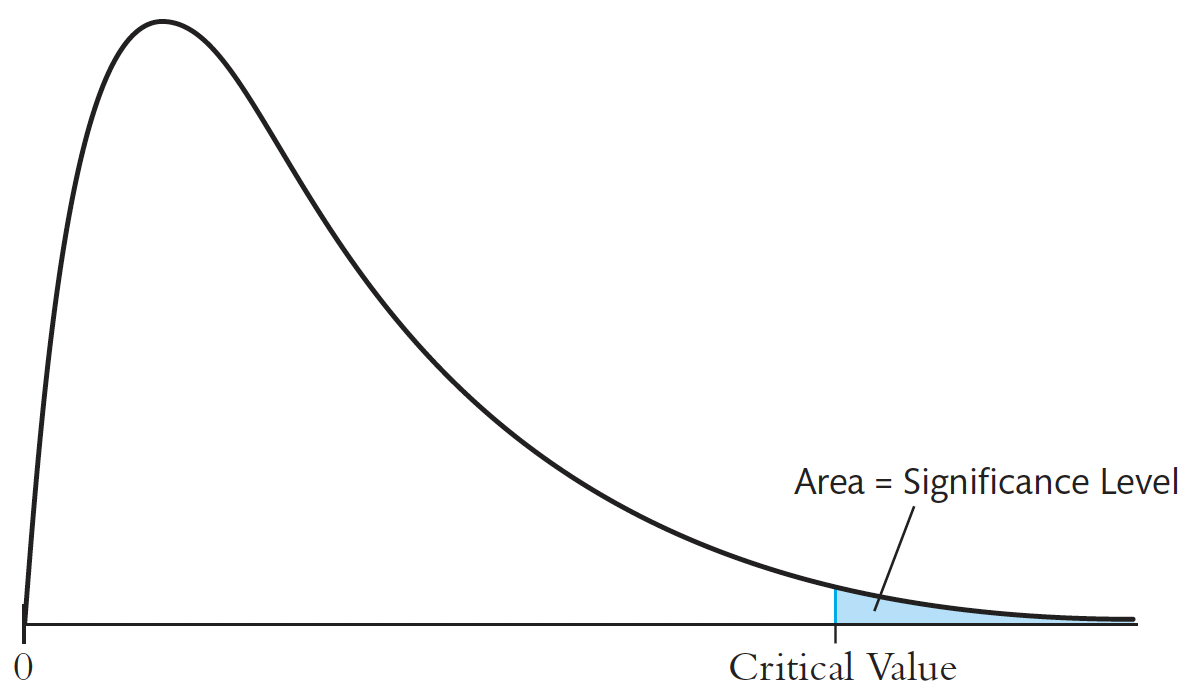
\includegraphics[scale=.6]{images/Fdist.png}
\end{figure}

\end{frame}






\begin{frame}{One Restriction: Why $F=t^2$}
\small
Test one restriction ($q=1$): $H_0:\beta_j=\beta_{j,0}$ against $H_1:\beta_j\neq\beta_{j,0}$.
\par\medskip
\textbf{1. Write the F-statistic for one restriction.}
\[F=\frac{(\hat\beta_j-\beta_{j,0})^2}{\widehat{\operatorname{Var}}(\hat\beta_j)}.\]
\textbf{2. A standard error is the square root of the estimated variance.}
\[\widehat{\operatorname{Var}}(\hat\beta_j)=[SE(\hat\beta_j)]^2.\]
\textbf{3. Substitute and recognize the t-statistic.}
\[F=\frac{(\hat\beta_j-\beta_{j,0})^2}{[SE(\hat\beta_j)]^2}
=\left[\frac{\hat\beta_j-\beta_{j,0}}{SE(\hat\beta_j)}\right]^2
=\boxed{t^2}.\]
$q=1$ means one restriction, even when the regression has several explanatory variables.
\end{frame}

\begin{frame}{Two t Tails Become One F Tail}
\small
For $q=1$, squaring maps both negative and positive t-statistics to $F\geq0$.
\begin{center}
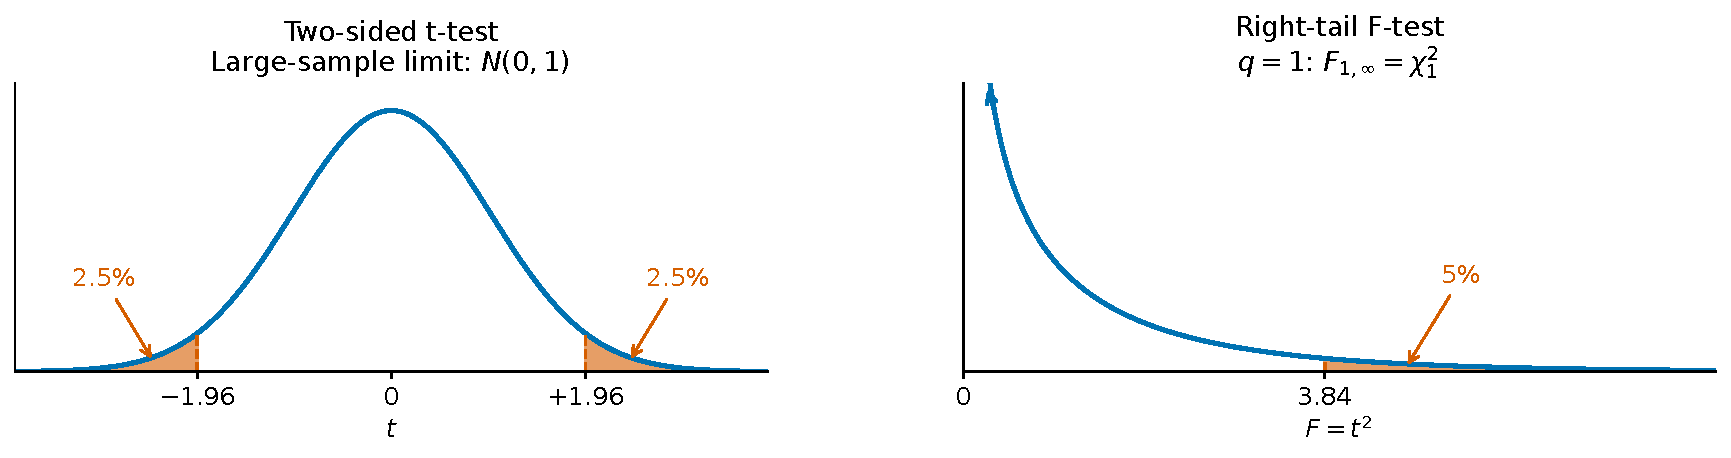
\includegraphics[width=.98\textwidth,height=.64\textheight,keepaspectratio]{images/lecture6_t_f_equivalence.pdf}
\end{center}
At the 5\% significance level, the two red t tails have total probability $2.5\%+2.5\%=5\%$, equal to the red right tail of F.
\[
 t<-1.96\ \text{or}\ t>1.96
 \quad\Longleftrightarrow\quad F=t^2>1.96^2\approx3.84.
\]
The alternative remains \textbf{two-sided}: large F detects a deviation in either direction.
\end{frame}

\begin{frame}{Why Squaring Combines the Two t Tails}
\small
Let $\nu=n-k-1$, where $k$ excludes the intercept.
\par\medskip
\textbf{Squaring removes the sign.} Let $a=|t_{\mathrm{obs}}|$.
\[
T_\nu^2\geq a^2
\quad\Longleftrightarrow\quad
T_\nu\leq-a\ \text{or}\ T_\nu\geq a.
\]
A squared value is at least $a^2$ whenever the original value is at least $a$ away from zero: in the left t tail or the right t tail.
\par\medskip
For $a>0$, these two events cannot overlap, so we add their probabilities:
\[
\underbrace{\Pr(T_\nu^2\geq a^2)}_{\text{one right tail after squaring}}
=
\underbrace{\Pr(T_\nu\leq-a)+\Pr(T_\nu\geq a)}_{\text{two t tails}}.
\]
\textbf{The same event in two forms:} squaring combines the two disjoint t tails into one right tail, without changing their total probability.
\end{frame}

\begin{frame}{\large Why the F-test and Two-Sided t-test Have the Same p-value}
\small
Under the null and the assumptions for exact t inference,
\[
T_\nu\sim t_\nu\quad\Longrightarrow\quad T_\nu^2\sim F_{1,\nu},
\qquad \nu=n-k-1.
\]
Therefore, the two tests count \textbf{the same null outcomes}:
\[
\boxed{\Pr(F_{1,\nu}\geq t_{\mathrm{obs}}^2)
=\Pr(|T_\nu|\geq |t_{\mathrm{obs}}|).}
\]
\textbf{Example: $\boldsymbol{t_{\mathrm{obs}}=-2}$, so $\boldsymbol{F_{\mathrm{obs}}=4}$.}
\[
F=T_\nu^2\geq4\quad\Longleftrightarrow\quad T_\nu\leq-2\ \text{or}\ T_\nu\geq2.
\]
\[
p_F=\Pr(F_{1,\nu}\geq4)
=\Pr(T_\nu\leq-2)+\Pr(T_\nu\geq2)
=p_{\text{two-sided t}}.
\]
The same reasoning gives $|t_{\mathrm{obs}}|>c\iff F_{\mathrm{obs}}>c^2$: square the two-sided t critical value to obtain the F critical value.
\par\smallskip
The next slide compares these critical values with the table on slide 12.
\end{frame}

\begin{frame}{The $q=1$ Row on Slide 12 Is the Squared t Table}
\small
Slide 12 reports \textbf{large-sample} F critical values. For one restriction, take the two-sided t cutoff (its standard-normal limit) and square it:
\[
 c_\alpha=\Phi^{-1}(1-\alpha/2),\qquad
 F_{1,\infty;1-\alpha}=c_\alpha^2.
\]
\begin{center}
\renewcommand{\arraystretch}{1.35}
\begin{tabular}{lrrr}
\hline
\textbf{Significance level $\alpha$} & \textbf{10\%} & \textbf{5\%} & \textbf{1\%}\\\hline
Two-sided t cutoff $c_\alpha$ & $1.644854$ & $1.959964$ & $2.575829$\\
Squared cutoff $c_\alpha^2$ & $2.705543$ & $3.841459$ & $6.634897$\\
\rowcolor[HTML]{DAE8FC}
F table, slide 12: $q=1$ & $\mathbf{2.71}$ & $\mathbf{3.84}$ & $\mathbf{6.63}$\\\hline
\end{tabular}
\end{center}
Square the unrounded quantile, then round the result: the highlighted values match slide 12 exactly.
\par\medskip
\textbf{Finite samples:} with matching $\nu=n-k-1$, the same relationship is
\[
 F_{1,\nu;1-\alpha}=\bigl(t_{\nu,1-\alpha/2}\bigr)^2.
\]
Only the $q=1$ row comes from a single squared t-statistic; $q>1$ tests several restrictions jointly.
\end{frame}

\begin{frame}{A Complete Example: Constructing $\hat\beta$ and $\widehat V$}
\footnotesize
\setlength{\abovedisplayskip}{4pt}
\setlength{\belowdisplayskip}{4pt}
Two regressors and an intercept: $Y_i=\beta_0+\beta_1X_{1i}+\beta_2X_{2i}+u_i$; $n=8$, $k=2$.
\par\medskip
\begin{columns}[T]
\begin{column}{.36\textwidth}
\textbf{All eight observations}
\[
X=\begin{pmatrix}
1&-1&-2\\
1&-1&-2\\
1&-1&0\\
1&-1&0\\
1&1&0\\
1&1&0\\
1&1&2\\
1&1&2
\end{pmatrix},\quad
Y=\begin{pmatrix}6\\8\\8\\10\\10\\12\\12\\14\end{pmatrix}.
\]
The first column of $X$ is for the intercept; the next two are $X_1$ and $X_2$.
\par\medskip
\textbf{Residuals and error variance}
\[
\hat u=Y-X\hat\beta=(-1,1,-1,1,-1,1,-1,1)'.
\]
\[
SSR=\hat u'\hat u=8,\qquad df=8-3=5,
\]
\[
SER^2=\frac{SSR}{n-k-1}=\frac85.
\]
\end{column}
\begin{column}{.61\textwidth}
\textbf{1. Form the cross-products.}
\[
X'X=\begin{pmatrix}8&0&0\\0&8&8\\0&8&16\end{pmatrix},\qquad
X'Y=\begin{pmatrix}80\\16\\24\end{pmatrix}.
\]
\textbf{2. Invert and multiply to obtain the OLS estimates.}
\[
(X'X)^{-1}=\frac18\begin{pmatrix}1&0&0\\0&2&-1\\0&-1&1\end{pmatrix},
\]
\[
\hat\beta=(X'X)^{-1}X'Y=(10,1,1)'.
\]
\textbf{3. Estimate the coefficient covariance matrix.}
\[
\widehat V=SER^2(X'X)^{-1}
=\frac15\begin{pmatrix}1&0&0\\0&2&-1\\0&-1&1\end{pmatrix}.
\]
Rows and columns follow $(\hat\beta_0,\hat\beta_1,\hat\beta_2)$.
For a joint test of the two slopes, use the bottom-right block:
\[
\widehat V_d=\begin{pmatrix}0.4&-0.2\\-0.2&0.2\end{pmatrix}.
\]
\end{column}
\end{columns}
\end{frame}

\begin{frame}{The F-statistic from Restricted and Unrestricted Fits}
The same F-statistic can be computed by comparing two OLS fits under the maintained assumptions.\\[1em]
\begin{enumerate}
\item Fit the restricted model, imposing $H_0$.\\[1em]
\item Fit the unrestricted model, which permits both the null and the alternative.\\[1em]
\item Compare their fit: if relaxing the restrictions improves fit sufficiently, reject $H_0$.
\end{enumerate}
\vspace{1em}
Use the same observations and outcome, an intercept in both models, and the same null hypothesis as in the coefficient formula.
\end{frame}

\begin{frame}{Example: Are the coefficients on $strs$ and $frpmfracs$ zero?}


Restricted population regression (that is, under $H_0$):
\begin{equation*}
    TestScore_i = \beta_0 + \beta_2 edfracbachplus_i + u_i
\end{equation*}
\\[1em]
Unrestricted population regression (permits both $H_0$ and $H_1$):
\begin{equation*}
    TestScore_i = \beta_0 + \beta_1 frpmfracs_i + \beta_2 edfracbachplus_i + \beta_3 strs_i + u_i
\end{equation*}
\\[1em]
The fit will be better (higher $R^2$) in the unrestricted regression. But by how much should it be higher for $strs$ and $frpmfracs$ to be deemed statistically significantly different from zero?
\end{frame}


\begin{frame}{The Same F-statistic from $R^2$}
\[F=\frac{(SSR_R-SSR_U)/q}{SSR_U/(n-k_U-1)}
=\frac{(R_U^2-R_R^2)/q}{(1-R_U^2)/(n-k_U-1)}.\]
\begin{itemize}
\item $R$ and $U$ denote restricted and unrestricted OLS fits.
\item $q$ is the number of restrictions; $k_U$ counts unrestricted regressors, excluding the intercept.
\item Use the same dataset and outcome, nested linear restrictions, and an intercept in both models.
\item $SER^2=SSR_U/(n-k_U-1)$ is the variance estimate used in the coefficient formula.
\item For $q=2$, this is exactly the two-coefficient formula shown earlier.
\end{itemize}
\vspace{.5em}
A greater improvement in fit gives a larger F-statistic.
\end{frame}


\begin{frame}{Example: Restricted and Unrestricted Fits}
\small
\setlength{\abovedisplayskip}{.35em}
\setlength{\belowdisplayskip}{.35em}
\textbf{Restricted fitted regression:}
\[\widehat{TestScore}_i=705.157+203.582\times edfracbachplus_i\]
\[R_R^2=1-\frac{SSR_R}{TSS_Y}=0.2320
\quad\Rightarrow\quad SSR_R=0.7680\,TSS_Y.\]
\textbf{Unrestricted fitted regression:}
\begin{align*}
\widehat{TestScore}_i={}&802.045-128.685\times frpmfracs_i\\
&+60.729\times edfracbachplus_i+0.564\times strs_i
\end{align*}
\[R_U^2=1-\frac{SSR_U}{TSS_Y}=0.4775
\quad\Rightarrow\quad SSR_U=0.5225\,TSS_Y.\]
Both fits use the same outcome and observations, so
$TSS_Y=\sum_i(Y_i-\bar Y)^2$ is the same.
\[\boxed{F=\frac{(R_U^2-R_R^2)/q}{(1-R_U^2)/(n-k_U-1)}}\]
$n=500$, $q=2$, $k_U=3$ ($k_U$ excludes the intercept).
\end{frame}

\begin{frame}{Example: Comparing the Two School Regressions}
\[F=\frac{(0.4775-0.2320)/2}{(1-0.4775)/(500-3-1)}=116.5244.\]
\begin{itemize}
\item There are $q=2$ restrictions and $500-3-1=496$ residual degrees of freedom.\\[1em]
\item Under the maintained assumptions and conditionally normal errors, use $F_{2,496}$ exactly; otherwise use a large-sample approximation.\\[1em]
\item The coefficient formula with the conventional covariance matrix gives the same F-statistic for these fits. The underlying data and covariance estimates are not provided here for a numerical verification.
\end{itemize}
\end{frame}


\begin{frame}{Worked Example: One Dataset, Two Formulas}
Constructed data: $n=8$, $k_U=2$. Test $H_0:\beta_1=\beta_2=0$ ($q=2$).
\begin{columns}[T]
\begin{column}{.35\textwidth}
\begin{center}
\begin{tabular}{rrrr}
\toprule
$i$&$X_1$&$X_2$&$Y$\\\midrule
1&-1&-2&6\\
2&-1&-2&8\\
3&-1&0&8\\
4&-1&0&10\\
5&1&0&10\\
6&1&0&12\\
7&1&2&12\\
8&1&2&14\\\bottomrule
\end{tabular}
\end{center}
\end{column}
\begin{column}{.62\textwidth}
\textbf{Unrestricted fit}
\[\widehat Y_i=10+X_{1i}+X_{2i}.\]
Residuals: $(-1,1,-1,1,-1,1,-1,1)$; $SSR_U=8$.\\[1em]
\textbf{Restricted fit}
\[\widehat Y_i=\bar Y=10,\qquad SSR_R=TSS_Y=48.\]
\[df=8-2-1=5,\qquad SER^2=\frac85.\]
\end{column}
\end{columns}
\end{frame}

\begin{frame}{Same Example: Coefficient-Based F}
The slope block of $\widehat V=SER^2(X'X)^{-1}$ is
\[\widehat V_s=\begin{pmatrix}2/5&-1/5\\-1/5&1/5\end{pmatrix}.\]
\[t_1=\frac1{\sqrt{2/5}}=\sqrt{5/2},\qquad
 t_2=\frac1{\sqrt{1/5}}=\sqrt5,\qquad
 \hat\rho=\frac{-1/5}{\sqrt{(2/5)(1/5)}}=-\frac1{\sqrt2}.\]
\[F=\frac12\frac{(5/2)+5-2(-1/\sqrt2)\sqrt{5/2}\sqrt5}{1-1/2}
=\boxed{12.5}.\]
The covariance term is essential: simply averaging $t_1^2$ and $t_2^2$ would give $3.75$, not the joint F-statistic.
\end{frame}

\begin{frame}{Same Example: Fit-Based F}
\[R_U^2=1-\frac8{48}=\frac56,\qquad R_R^2=0.\]
\[F=\frac{(5/6-0)/2}{(1-5/6)/5}=12.5,\qquad
F=\frac{(48-8)/2}{8/5}=12.5.\]
\[\boxed{F_{\text{coefficient formula}}=F_{\text{fit formula}}=12.5}\]
With conditionally normal errors, the exact null reference is $F_{2,5}$:
\[p=\Pr(F_{2,5}\geq12.5)=\left(\frac16\right)^{5/2}=.01134023.\]
Both formulas give the same p-value and reject at 5\%. Without normality, inference uses a large-sample approximation, which need not be accurate at $n=8$.
\end{frame}


\begin{frame}{Testing Single Restrictions on Multiple Coefficients}
Consider the following specification
\begin{equation*}
    Y_i = \beta_0 + \beta_1 X_{1i}+ \beta_2 X_{2i} +u_i
\end{equation*}
and the null and alternative hypothesis,
\begin{eqnarray*}
    H_0 := \beta_1=\beta_2 \text{~~VS~~}  & H_1 &:= \beta_1\neq\beta_2
\end{eqnarray*}
This null imposes a single restriction on multiple coefficients – it is not a joint hypothesis with multiple restrictions!\\[1em]

Here are two methods for testing single restrictions on multiple coefficients:
\begin{enumerate}
    \item Rearrange the regressors so that the restriction becomes a restriction on a single coefficient in an equivalent regression; or,
    \item Perform the test directly (Some software, including STATA, lets you test restrictions using multiple coefficients directly)
\end{enumerate}
\end{frame}


\begin{frame}{Rearranging}
From the following specification
\begin{equation*}
    Y_i = \beta_0 + \beta_1 X_{1i}+ \beta_2 X_{2i} +u_i
\end{equation*}
Add and substract $ \beta_2 X_{1i}$:
\begin{eqnarray*}
    &Y_i &= \beta_0 + (\beta_1 - \beta_2)X_{1i}+ \beta_2 (X_{2i} + X_{1i}) +u_i\\
    & &= \beta_0 + \gamma_1 X_{1i}+ \beta_2 W_{i} +u_i
\end{eqnarray*}
Then test:
\begin{eqnarray*}
    H_0 := \gamma_1=0 \text{~~VS~~}  & H_1 &:= \gamma_1\neq 0
\end{eqnarray*}
The original and rearranged regressions have the same $R^2$, the same predicted values, and the same residuals, but the problem is now a simpler one.
\end{frame}


\begin{frame}{Testing Equality Using the Same Example}
Test $H_0:\beta_1=\beta_2$, a single restriction ($q=1$).
\[\hat d=\hat\beta_1-\hat\beta_2=1-1=0.\]
\begin{align*}
\widehat{\operatorname{Var}}(\hat d)
&=\widehat{\operatorname{Var}}(\hat\beta_1)+\widehat{\operatorname{Var}}(\hat\beta_2)
-2\widehat{\operatorname{Cov}}(\hat\beta_1,\hat\beta_2)\\
&=.4+.2-2(-.2)=1.
\end{align*}
\[SE(\hat d)=1,\qquad t=\frac01=0,\qquad F=t^2=0.\]
Under the exact normal-error reference ($t_5$ or $F_{1,5}$), $p=1$: do not reject equality. The same conventional covariance matrix is used throughout.
\end{frame}


\begin{frame}{Confidence Sets for Multiple Coefficients}
Consider the following regression
\begin{equation*}
    Y_i = \beta_0 + \beta_1 X_{1i} + \beta_2 X_{2i} + \dots  + \beta_k X_{ki} + u_i
\end{equation*}\\[1em]

What is a joint confidence set for $\beta_1$ and $\beta_2$?\\[1em]

A 95\% joint confidence set is:
\begin{itemize}
    \item A set-valued function of the data that contains the true coefficients in approximately 95\% of repeated samples, using our large-sample approximation.
    \item Equivalently, the set of coefficient values that cannot be rejected at the 5\% significance level
\end{itemize}

You can find a 95\% confidence set as the set of $(\beta_1, \beta_2)$ that cannot be rejected at the 5\% level using an F-test (why not just combine the two 95\% confidence intervals?).

\end{frame}


\begin{frame}{Confidence Sets for Multiple Coefficients}
\begin{itemize}
\item Let $F(\beta_{1,0},\beta_{2,0})$ test $H_0:\beta_1=\beta_{1,0},\ \beta_2=\beta_{2,0}$ using the conventional covariance matrix.\\[1em]
\item The 95\% confidence set is
\[\{(\beta_{1,0},\beta_{2,0}):F(\beta_{1,0},\beta_{2,0})\le c\},
\qquad c=F_{2,\infty;.95}\approx3.00.\]
\item We use the large-sample critical value from the F table on slide 12.\\[1em]
\item The resulting joint confidence set has approximately 95\% coverage in repeated samples.\\[1em]
\item Inverting a 5\% test includes precisely the coefficient pairs that are not rejected.
\end{itemize}
\end{frame}


\begin{frame}{Reminder: A Confidence Set for One Coefficient}
\small
\setlength{\abovedisplayskip}{4pt}
\setlength{\belowdisplayskip}{4pt}
\begin{enumerate}
\item \textbf{Test each candidate value.} For $H_0:\beta_j=b$ vs.\ $H_1:\beta_j\ne b$, define
\[
t(b)=\frac{\hat\beta_j-b}{SE(\hat\beta_j)}.
\]
Under $H_0$, this statistic is approximately $N(0,1)$ in large samples: the two-sided 5\% cutoff is $1.96$.
\item \textbf{Keep every value not rejected at 5\%:}
\[
\{b\in\mathbb{R}:|t(b)|\le1.96\}
=\left\{b\in\mathbb{R}:\left|\frac{\hat\beta_j-b}{SE(\hat\beta_j)}\right|\le1.96\right\}.
\]
\item \textbf{Rearrange to obtain the familiar interval:}
\[
|\hat\beta_j-b|\le1.96\,SE(\hat\beta_j)
\iff \hat\beta_j-1.96\,SE(\hat\beta_j)\le b\le\hat\beta_j+1.96\,SE(\hat\beta_j).
\]
\[
\boxed{\bigl[\hat\beta_j-1.96\,SE(\hat\beta_j),\ \hat\beta_j+1.96\,SE(\hat\beta_j)\bigr].}
\]
\end{enumerate}
This is an approximate 95\% confidence interval: over repeated samples, about 95\% of the intervals constructed this way contain the true $\beta_j$.

\medskip
For one coefficient, the set is an interval; for two coefficients, the joint set is a region of pairs.
\end{frame}


\begin{frame}{Confidence Sets for Multiple Coefficients}
For each candidate pair, define
\[t_1=\frac{\hat\beta_1-\beta_{1,0}}{SE(\hat\beta_1)},\qquad
 t_2=\frac{\hat\beta_2-\beta_{2,0}}{SE(\hat\beta_2)}.\]
The confidence set uses the same coefficient formula:
\[\left\{(\beta_{1,0},\beta_{2,0}):
\frac{t_1^2+t_2^2-2\hat\rho t_1t_2}{2(1-\hat\rho^2)}\le c\right\},
\qquad c=F_{2,\infty;.95}\approx3.00.\]
The cross term is $-2\hat\rho t_1t_2$. The boundary is obtained by setting $F=c$; the confidence set includes the boundary and its interior.\\[1em]
The next slide rewrites this boundary as the equation of an ellipse.
\end{frame}


\begin{frame}{Why the Boundary $F=c$ Is an Ellipse}
\small
\setlength{\abovedisplayskip}{4pt}
\setlength{\belowdisplayskip}{4pt}
\textbf{1. Start from the boundary and rotate the axes.}
\[
t_1^2+t_2^2-2\hat\rho t_1t_2=2c(1-\hat\rho^2),\qquad
z_1=\frac{t_1+t_2}{\sqrt2},\quad z_2=\frac{t_2-t_1}{\sqrt2}.
\]
These new coordinates follow the two diagonal directions in the $(t_1,t_2)$ plane.
\par\smallskip
\textbf{2. Substitute to remove the cross term.}
\[
t_1^2+t_2^2=z_1^2+z_2^2,\qquad 2t_1t_2=z_1^2-z_2^2,
\]
\[
\underbrace{(1-\hat\rho)z_1^2+(1+\hat\rho)z_2^2}_{t_1^2+t_2^2-2\hat\rho t_1t_2}
=2c(1-\hat\rho^2).
\]
\textbf{3. Divide to obtain the standard ellipse equation.}
\[
\boxed{\frac{z_1^2}{2c(1+\hat\rho)}+\frac{z_2^2}{2c(1-\hat\rho)}=1.}
\]
Both denominators are positive when $|\hat\rho|<1$. This has the familiar form $z_1^2/a^2+z_2^2/b^2=1$, with semiaxes $a=\sqrt{2c(1+\hat\rho)}$ and $b=\sqrt{2c(1-\hat\rho)}$.
\par\smallskip
Rotating back to $(t_1,t_2)$ and rescaling by the standard errors gives an ellipse in coefficient values, centered at $(\hat\beta_1,\hat\beta_2)$, where $t_1=t_2=0$.
\end{frame}


\begin{frame}{Confidence Sets for Multiple Coefficients}
\begin{figure}
  \centering
         \vspace{-1mm}
         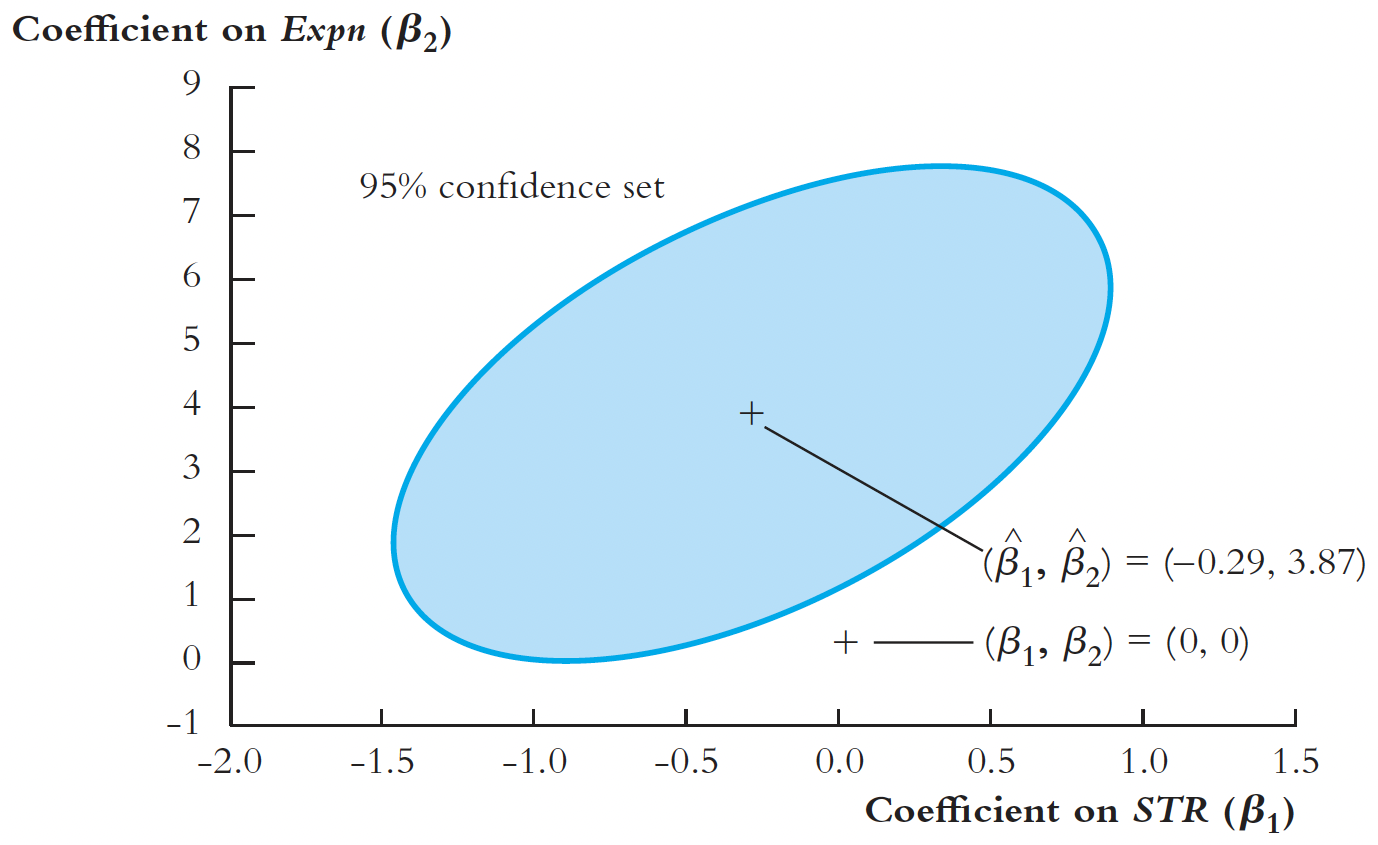
\includegraphics[scale=.5]{images/multireg_ci.png}
\end{figure}
\end{frame}


\begin{frame}{How to decide what variables to include}
\begin{enumerate}
    \item Identify the variable of interest

    \item Think of the omitted causal effects that could result in omitted variable bias

    \item Include those omitted causal effects if you can or, if you can’t, include variables correlated with them that serve as control variables.

    \begin{itemize}
        \item The control variables are effective if the conditional mean independence assumption plausibly holds, that is, if $u$ is uncorrelated with the share of subsidized meals once the control variables are included. 
        \item This results in a “base” or “benchmark” model.
    \end{itemize}

    \item Also specify a range of plausible alternative models, which include additional candidate variables.

    \item Estimate your base model and plausible alternative specifications (“sensitivity checks”).
    \begin{itemize}
        \item Does a candidate variable change the coefficient of interest $\beta_1$?
        \item Is a candidate variable statistically significant?
        \item Use judgment, not a mechanical recipe…
        \item Don’t just try to maximize the $R^2$ !
    \end{itemize}
\end{enumerate}
\end{frame}

\begin{frame}{What the $R^2$ tells you, and what it doesn't }
It is easy to fall into the trap of maximizing the $R^2$ and $\overline{R}^2$ but this loses sight of our real objective: an unbiased estimator of the class size effect.\\[1em]
\begin{itemize}
    \item A high $R^2$ (or $\overline{R}^2$) means that the regressors explain the variation in your data\\[1em]
    \item A high $R^2$ (or $\overline{R}^2$) \textbf{does not} mean that you have eliminated omitted variable bias
    \item A high $R^2$ (or $\overline{R}^2$) \textbf{does not} mean that you have an unbiased estimator of a causal effect $\beta_1$
    \item A high $R^2$ (or $\overline{R}^2$) \textbf{does not} mean that the included variables are statistically significant --- this must be determined using hypotheses tests.
\end{itemize}
\end{frame}

\begin{frame}{Summary}
\begin{itemize}
    \item Multiple regression allows you to estimate the effect on $Y$ of a change in $X_1$, holding other included variables constant.\\[1em]
    \item If you can measure a variable, you can avoid omitted variable bias from that variable by including it.\\[1em]
    \item If you can’t measure the omitted variable, you still might be able to control for its effect by including a control variable.\\[1em]
    \item There is no simple recipe for deciding which variables belong in a regression -- you must exercise judgment.\\[1em]
    \item One approach is to specify a base model -- relying on a priori reasoning -- then explore the sensitivity of the key estimate(s) in alternative specifications.
\end{itemize}

\end{frame}



\begin{frame}[allowframebreaks]{Material}
\begin{itemize}
    \item[--] \textbf{Textbooks:}
    \begin{itemize}
        \item Introduction to Econometrics, 4th Edition, Global Edition, by Stock and Watson -- Chapter 7
    \end{itemize}
\end{itemize}
\end{frame}




\end{document}
